\section{Kvantitativ beskrivning av energiflöden}

Genom att beräkna storlekarna energiflödena genom byggnadens olika delar kan vi se var energiflödena är som störst vid olika väderförhållanden. Vi har valt att titta på en klar dag i mitten av april då solinstrålningen når en topp vid $\unit[640]{W/m^2}$ och solen är uppe i 14 timmar. Dygnets temperatur varierar mellan $\unit[6]{^\circ C}$ och $\unit[9]{^\circ C}$ och vinden är runt $\unit[10]{m/s}$. Enligt väderstatistik från SMHI bör detta vara en rimlig dag med väldigt bra väder vid den valda tiden på året.

Vi vald en dag med fint väder eftersom energiflödena då är små och kan de förbättras när de är små, kan de också förbättras när de är stora. Att vi valde en dag i april beror på att det fortfarande är under eldningssäsongen, det vill säga den tid på året då man fortfarande värmer upp huset. Eldningssäsongen för fastigheten på Walleriusgatan är ungefär från början oktober till slutet av april. Under sommaren sker ingen uppvärmning.

\section{Kvantifiering av konstanta energiflöden}

Flera av energiflödena genom fastigheten är relativt konstanta sett till en längre tidsperiod. Det gäller främst värme från elektriska apparater, så som kylskåp och datorer, människors kroppsvärme och varmvattencirkulation. På så sätt kan aktivt tillförd energi, det vill säga den energitillförsel som kan regleras och tillförs via radiatorerna, enkelt regleras med hänsyn till dessa, om man bara känner dess storlek.

\subsection{Uppvärmning från människor}
Den utstrålade kroppsvärmen från människor kan beräknas genom att de antas vara svartkroppar. Stefan-Boltzmanns lag säger då att utstrålade energi per yt- och tidsenhet är $j=\sigma T^4$, där $T$ är temperaturen och $\sigma=\unit[5.6705\cdot 10^8]{Wm^{-2}K^{-4}}$ \cite{physicshandbook}, se teoriavsnitt \ref{sec:blackbody}. På samma sätt beräknas den energi som strålas in mot kroppen från omgivningen. Nettostrålningen från en människa kan då ses i ekvation \eqref{eq:constantsources:stefan} där $T_k=37^{\circ}C=310K$ är kroppstemperaturen och $T_r=20^{\circ}C=293K$ är rumstemperaturen. Multipliceras det med en människas area, ungefär $\unit[2]{m^2}$, fås en nettoeffekt på $\unit[211]{W}$. I själva verket reduceras denna effekt av en rad faktorer. Exempelvis är hudens temperatur lägre än kroppstemperaturen samtidigt som klädesplagg reducerar effektutstrålningen något. Professor Göran Grimvall skriver i NyTeknik att en rimlig nettoeffekt vid vila är cirka 1 W per kilogram kroppsvikt, alltså ungefär $\unit[50-100]{W}$\cite{Grimvall}.

\begin{equation}
\label{eq:constantsources:stefan}
j=\sigma \left( T_k^4 - T_r^4 \right)
\end{equation}
\noindent

\subsection{Varmvattencirkulation i fastigheten}
I huset cirkulerar hela tiden varmvattnet för att alltid kunna tillgodose de boendes behov av varmvatten utan dröjsmål. Efter en tur i systemet sjunker temperaturen på varmvattnet med tre grader och flödet är $\unit[800]{l/h}$. Detta motsvarar en energitillförsel till fastigheten på $\unit[2,8]{kW}$.

\subsection{Energi från elektrisk apparatur}
Den största delen av energin som driver en elektrisk apparat blir till värme. Därför låter vi energiflödet från elektriska apparatur motsvaras av fastighetens energiförbrukning, vilken kan läsas av kontinuerligt och på så sätt bli en del av reglersystemet.



\subsection{Energiflöde genom väggar}

Hur värmen sprider, eller inte sprider, sig genom en vägg beror på dess material och temperaturerna på vardera sidan av väggen. I fallet när ena sidan av väggen befinner sig utomhus beror spridning också av solinstrålningen och hur mycket det blåser från olika håll. För detta har en modell satts upp utifrån vilken det har gjorts beräkningar av storleken på energiflödet genom väggen under ett dygn då mängden moln är konstant. En modell för hur energiflödet skulle förändras vid ett väderomslag har också satts upp. Båda modellerna har sedan används för både en oisolerad vägg bestående enbart av 50 cm tegel och en vägg isolerad med 10 cm mineralull.

Slutligen har det gjorts beräkningar på hur stora tryckskillander en vind som är ortogonal mot väggen ger upphov till. Dessa tryckförändringar driver luft att färdas genom otätheter i huset och drag uppstår vilket ger ett energiflöde genom väggen vid olika inom- och utomhustemperaturer.

\subsection{Flöde vid termisk jämvikt}
\label{sec:steadystatewall}

%To regerenate the figures use /code/pdesolver/generateWallFigApril.m
%with the argument /code/pdesolver/walldata.mat

För att visualisera flödet genom en vägg vid konstant väder och utomhustemperatur görs 
beräkningar med finita elementmetoden och en konstant inomhustemperatur på 
$\unit[20]{^\circ C}$. Utomhusvädret är relativt konstant och är satt till antingen molnig 
eller klart en dag i april då utomhustemperaturen varierar mellan $\unit[6]{^\circ C}$ på natten och $\unit[9]{^\circ C}$ på dagen. Detta har gjorts för en vägg utan isolering och en vägg med 
isolering, se figur~\ref{fig:energyflow_stst}. Den oisolerade väggen består av 
$\unit[0,5]{m}$ tegel och den isolerade har dessutom $\unit[0,1]{m}$ mineralull. 

\begin{figure}[hpbt]
\centering

\subfloat[Energiflöde ut från insidan av en oisolerad vägg en klar dag i april.]{
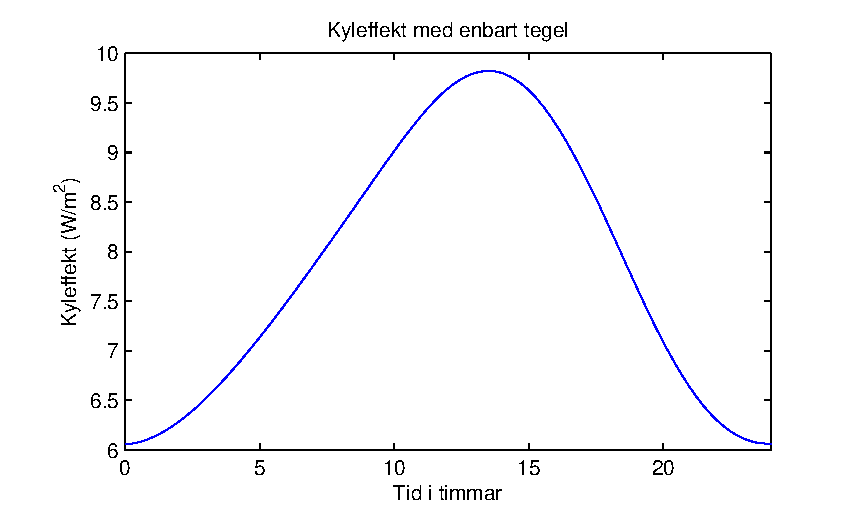
\includegraphics[width=6cm]{images/noinsulationapril.eps}}\vspace{1cm}
\subfloat[Energiflöde ut från insidan av en isolerad vägg en klar dag i april.]{
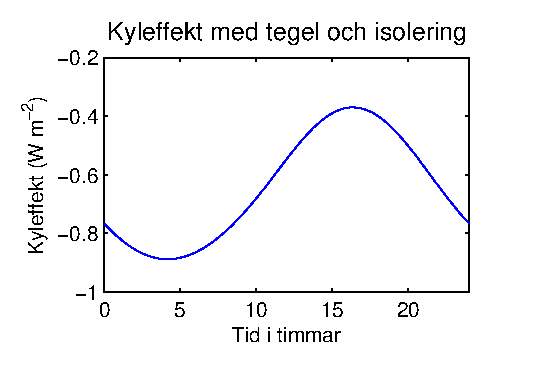
\includegraphics[width=6cm]{images/insulationapril.eps}
}

\subfloat[Energiflöde ut från insidan av en oisolerad vägg en molnig dag i april.]{
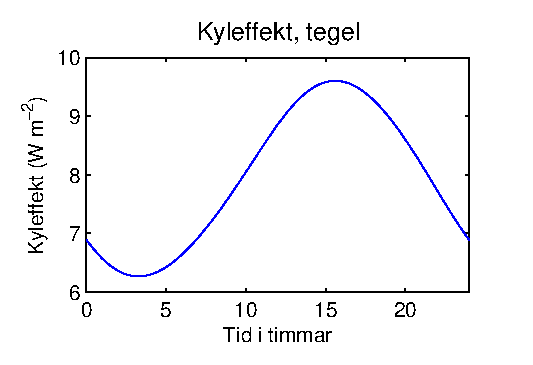
\includegraphics[width=6cm]{images/noinsulationcloud.eps}}\vspace{1cm}
\subfloat[Energiflöde ut från insidan av en isolerad vägg en molnig dag i april.]{
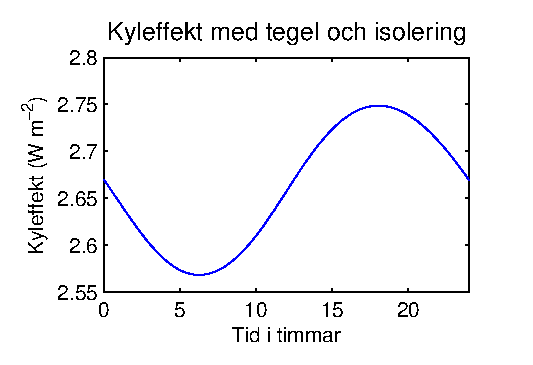
\includegraphics[width=6cm]{images/insulationcloud.eps}
}

\caption{\label{fig:energyflow_stst} Energiflöden ut från insidan av en vägg en dag i mitten av april. Utflöden ut genom väggen betecknas positivt, och inflöden negativt. }
\end{figure}


%RESULTAT ur graferna 
I figur \ref{fig:energyflow_stst} kan vi se att energiflödet genom väggen minskar till 
ungefär en fjärdedel med isolering. Under ett soligt dygn kommer det att flöda värme in i
 fastigheten. På grund av fördröjningen i väggen sker detta främst under natten, 
 och mindre på dagen. Med isolering blir energiflöde mindre och jämnare och inflödet når aldrig över $\unit[1]{W~m^{-2}}$.

Under en molnig dag med samma temperatur varierar energiflödet mellan $6$ och $10$ 
$\unit{W~m^{-2}}$ utan isolering. Med isolering minskar det till att röra sig mellan $1,9$ och $2,2$ $\unit{W~m^{-2}}$ ut ur 
fastigheten. En isolering innebär en molnig aprildag ett minskat energiutflöde och därmed en minskad 
energiförlust för fastigheten.

Trots att energi flödar in i fastigheten den klara dygnet så flödar ganska mycket energi 
ut ur fastigheten under det molniga dygnet. Göteborg har 1800 soltimmar under ett
 år av de totalt 4380 timmar som solen är över horisonten. Utifrån SMHI:s väderstatistik \cite{SMHIdata}
 kan beräknas att ungefär 37\% av dessa sker under eldningssäsongen, oktober till april. 
 Detta motsvarar ungefär 8\% av dygnets alla timmar. Tyvärr så förlorar fastigheten mer 
 energi än vad den tjänar på att inte isoleras utslaget på hela eldningssäsongen.

Under en fin sommardag kan det också tänkas att fastigheten värms över den önskade 
temperaturen och energi istället måste läggas på kylning. Med en isolering minskas även 
effekten av detta och energiflödena blir mindre och jämnare.

%%%%%%%%%%%%%%%%%%%%%%%%%%%%%%%%%%%%%%%%%%%%
\paragraph{En decemberdag}

Vidare har också energiflödena genom väggen en kall decemberdag undersökts, 
alltså en dag där energiflödena bör bli ganska stora. Detta kan ses som en övre uppskattning på fastighetens energiåtgång. Två fall av
denna dag har undersökts, dels en molning dag och dels en klar dag.

 Temperaturen går från $\unit[-5]{^\circ C}$ på dagen till $\unit[-11]{^\circ C}$. 
 Konvektionskoefficienten har satts till $h=\unit[35]{W~m^{-2}~K^{-1}}$ 
 vilket motsvarar en vindhastighet $\unit[7]{m~s^{-1}}$ parallellt med väggens yta. 
 Beräkningarna är genomförda genom att väggens tvärsnitt approximerats med en stav och sedan behandlats med finita elementmetoden.


\begin{figure}[hpbt]
\centering
\subfloat[Energiflöde ut från insidan av en oisolerad vägg en molnig dag i december.]{
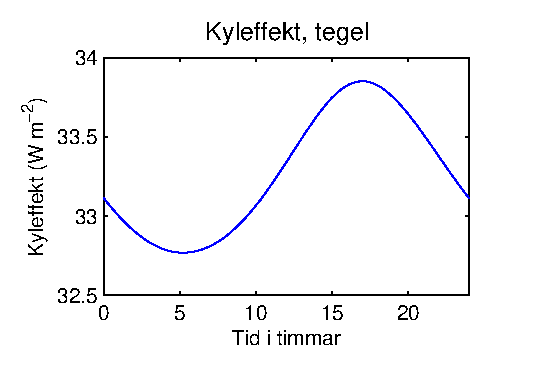
\includegraphics[width=6cm]{images/noinsulationdec.eps}}
\subfloat[Energiflöde ut från insidan av en isolerad vägg en molnig dag i december..]{
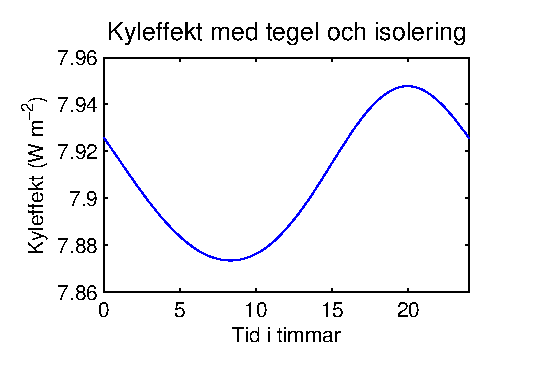
\includegraphics[width=6cm]{images/insulationdec.eps}
}

\subfloat[Energiflöde ut från insidan av en oisolerad vägg en klar dag i december.]{
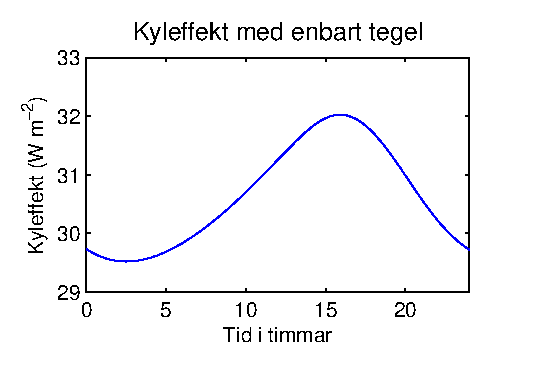
\includegraphics[width=6cm]{images/decsunnoinsulation.eps}
}\vspace{1cm}
\subfloat[Energiflöde ut från insidan av en isolerad vägg en klar dag i december.]{
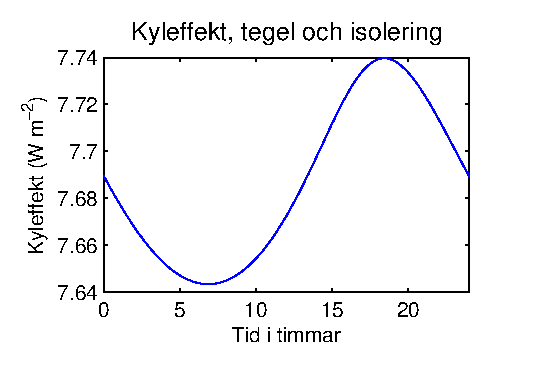
\includegraphics[width=6cm]{images/decsuninsulation.eps}
}

\caption{\label{fig:wall_dec} Energiflöden ut från insidan av en vägg en dag i december Utflöden ut genom väggen betecknas positivt, och inflöden negativt. 
}
\end{figure}

% Resultat
Även i december blir energiflödet genom en isolerad vägg ungefär en fjärdedel av det 
genom en oisolerad vägg, se figur~\ref{fig:wall_dec}. Här minskar det dock från ungefär $33,5$ 
till $\unit[8,05]{W~m^{-2}}$ ut ur väggen för den molniga dagen och från ungefär $32$ till $7,7$ $\unit{W~m^{-2}}$ den soliga dagen. Vi ser också i figurerna att energiflödet också blir 
jämnare med isolering – det varierar med mindre än $\unit[0,1]{W~m^{-2}}$ över dygnet, 
istället för drygt $\unit[1]{W~m^{-2}}$ utan isolering. Det gäller både vid klart och mulet väder. Detta är eftersträvansvärt om en jämn inomhustemperatur önskas. Energiflödet påverkas inte lika mycket av solen på vintern som under den varmare delen av året. En dag i december finns det betydligt mindre att tjäna på att inte isolera och hoppas att solen skiner, jämfört med en dag i april.

%%%% BURSPRÅK %%%%%%%%%%%%%%%%%%%%%%%%%%%%%%%
\paragraph{Burspråket}

Burspråket är inte uppbyggt av tegel, som de andra väggarna, utan av gips, isolering och koppar på spånskiva, se avsnitt~\ref{subsec:walls}. Energiflödet i burspråket visas här för alla fyra fallen: klar och molnig aprildag samt klar och molnig decemberdag.

\begin{figure}[hpbt]
\centering
\subfloat[\label{fig:bursprak_april1} Energiflöde ut från insidan av burspråket en klar dag i april.]{
	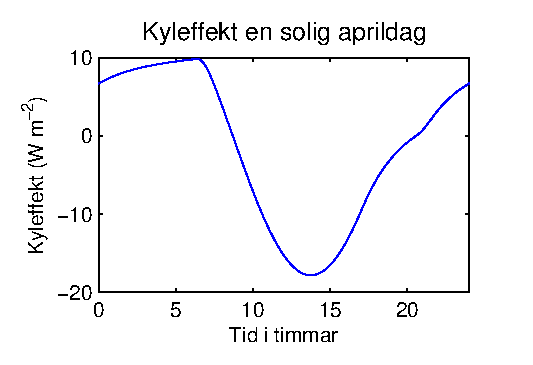
\includegraphics[width=6cm]{images/baysunapril.eps}
}
\subfloat[\label{fig:bursprak_april2} Energiflöde ut från insidan av burspråket en molnig dag i april.]{
	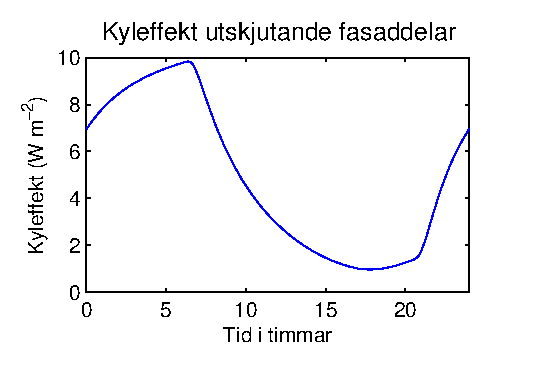
\includegraphics[width=6cm]{images/baynosunapril.eps}
}

\subfloat[\label{fig:bursprak_decsun} Energiflöde ut från insidan av burspråket en klar dag i december.]{
  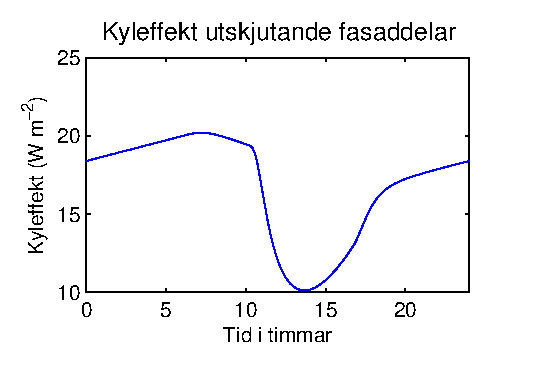
\includegraphics[width=6cm]{images/decsunbay.eps}
}
\subfloat[\label{fig:bursprak_dec} Energiflöde ut från insidan av burspråket en molnig dag i december.]{
	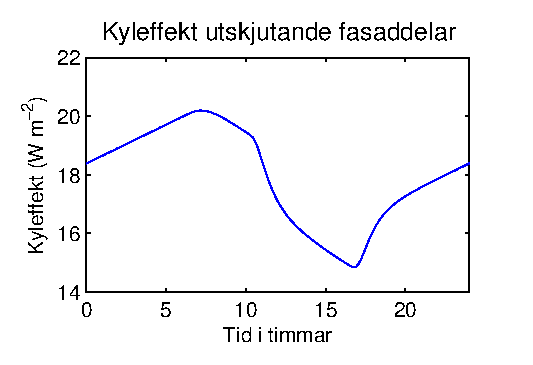
\includegraphics[width=6cm]{images/baynosundec.eps}
}
\caption{\label{fig:bursprak_energi} Energiflöden ut från insidan av en vägg. Utflöden ut genom burspråket betecknas positivt, och inflöden negativt. }
\end{figure}

Genom burspråket ser energiflödet lite annorlunda ut jämfört med det genom tegelväggarna,
se figur~\ref{fig:bursprak_energi}. En aprilmorgon innan solen har gått upp når energiflöde
sitt maximum med $\unit[10]{W~m^{-2}}$. När solen sedan värmer burspråket börjar energi
istället flöda in i byggnaden och en riktigt solig dag är det maximala inflödet över
$\unit[20]{W~m^{-2}}$, se figur~\ref{fig:bursprak_april1}. En molnig dag stannar det istället på ungefär $\unit[1]{W~m^{-2}}$ ut ur burspråket, se figur~\ref{fig:bursprak_april2}

En molnig dag i december är det betydligt kallare och energiutflödet varierar mellan 16 och
$\unit[21]{W~m^{-2}}$, se figur~\ref{fig:bursprak_dec}. En solig decemberdag är det tyvärr
inte mycket bättre och kyleffekten är alltid större än $\unit[10]{W~m^{-2}}$, se
figur~\ref{fig:bursprak_decsun}.
En intressant detalj är att kyleffekten på burspråket inte alls är sinusformad, på det vis som flödet genom väggarna i figur~\ref{fig:energyflow_stst} och \ref{fig:wall_dec} är. Det beror troligen på att burspråkets väggar är väldigt tunna och reagerar snabbt på förändringar.

%%%%%%%%TAKET%%%%%%%%%%%%%%%%%%%%%%%%%%%%%%%
\paragraph{Taket}


Energiflödet genom taket beräknas på samma sätt som energiflödet genom väggarna. Skillnaden, förutom materialet, är takets vinkel mot solen. I figur~\ref{fig:rooffiguressun} visas energiflödet för en solig april- respektive decemberdag. Eftersom taket lutar har nordsidan och sydsidan olika flöden ty solen skiner olika mycket på de olika lutade ytorna. Figur \ref{fig:rooffigurescloud} visar i sin tur situationen på molniga dagar, då ingen direkt solstrålning faller på taket.



\begin{figure}[hpbt]
\centering
\subfloat[\label{fig:roofaprilsunsouth} Energiflöde ut från insidan av sydsidan av taket en klar dag i april.]{
	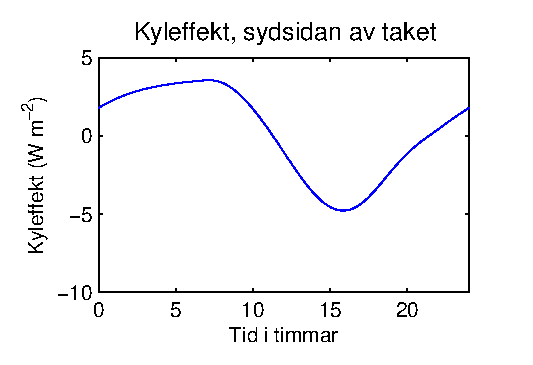
\includegraphics[width=6cm]{images/roofaprilsunsouth.eps}
}
\subfloat[\label{fig:roofaprilsunnorth}Energiflöde ut från insidan av norrsidan av taket en klar dag i april.]{
	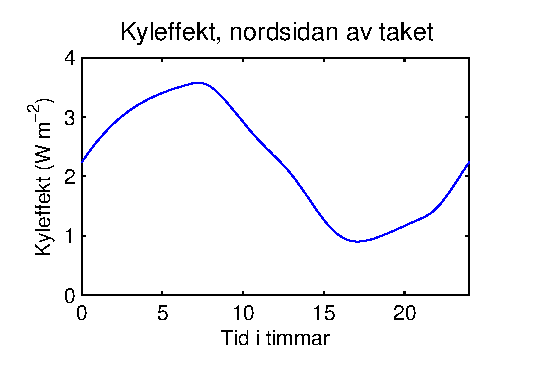
\includegraphics[width=6cm]{images/roofaprilsunnorth.eps}
}

\subfloat[\label{fig:roofdecsunsouth} Energiflöde ut från insidan av sydsidan av taket en klar dag i december.]{
	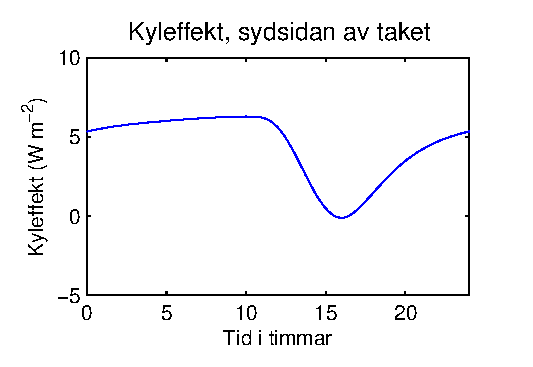
\includegraphics[width=6cm]{images/roofdecsunsouth.eps}
}
\subfloat[\label{fig:roofdecsunnorth} Energiflöde ut från insidan av nordsidan av taket en molnig dag i december.]{
	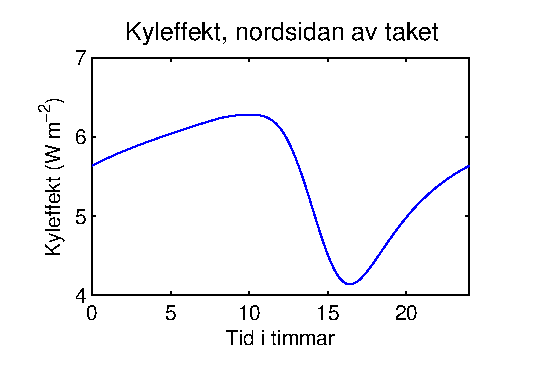
\includegraphics[width=6cm]{images/roofdecsunnorth.eps}
}

\caption{\label{fig:rooffiguressun}Energiflöden ut från insidan av en taket, klara dagar. Utflöden ut genom taket betecknas positivt, och inflöden negativt. }
\end{figure}

\begin{figure}[hpbt]
\centering
\subfloat[\label{fig:roofaprilnosun} Energiflödet från insidan av taket en molnig aprildag.]{
	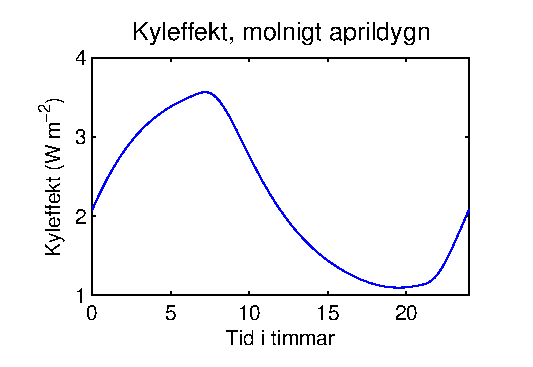
\includegraphics[width=6cm]{images/roofaprilnosun.eps}
}
\subfloat[\label{fig:roofdecnosun} Energiflödet från insidan av taket en molnig decemberdag.]{
	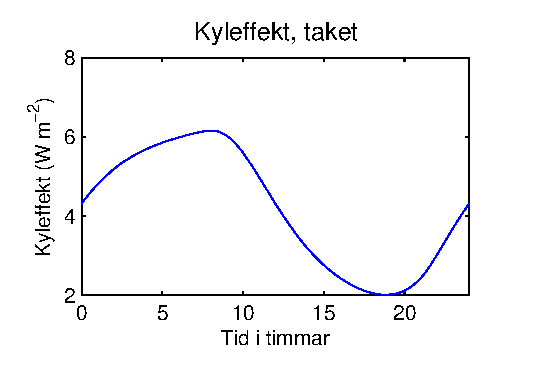
\includegraphics[width=6cm]{images/roofdecnosun.eps}
}

\caption{\label{fig:rooffigurescloud}Energiflöden ut från insidan av en taket, soliga dagar. Utflöden ut genom taket betecknas positivt, och inflöden negativt.}
\end{figure}

Energiflödet genom taket 
en klar dag i april varierar mellan $\unit[9]{W~m^{-2}}$ in och $\unit[3]{W~m^{-2}}$ ut på sydsidan, se figur~\ref{fig:roofaprilsunsouth}, 
och 
mellan $\unit[1]{W~m^{-2}}$ in och $\unit[3]{W~m^{-2}}$ ut på nordsidan, se figur~\ref{fig:roofaprilsunnorth}. 
Detta kan vidare jämföras med en molnig aprildag där utflödet varierar ännu mindre, bara mellan 0 och $\unit[3,5]{W~m^{-2}}$, se figur~\ref{fig:roofaprilnosun}. Solen har alltså stor en påverkan på energiflödets variationer.

En klar dag i december varierar energiflödet mellan 0 och drygt $\unit[5]{W~m^{-2}}$ ut ur taket på sydsidan och mellan drygt $\unit[4]{W~m^{-2}}$ och drygt $\unit[6]{W~m^{-2}}$ ut ur taket på nordsidan, se figur~\ref{roofdecsunsouth.eps} och \ref{roofdecsunnorth.eps}. En molnig dag i december varierar energiutflödet mellan 2 och $\unit[6]{W~m^{-2}}$, se figur~\ref{fig:roofdecnosun},


%%%%%%%%%%%%%%%%%%%%%%%%%%%%%%%%%%%%%%%%%%%%


\subsubsection{Flöde vid transient förlopp}

%To regerenate the figures use /code/pdesolver/calculateRisetime.m
%with the argument /code/pdesolver/wallstep.mat

\begin{figure}[hpbt]
\centering

\subfloat[Energiflöde ut från insidan av en vägg med $0,5\mbox{m}$ tegel.]{
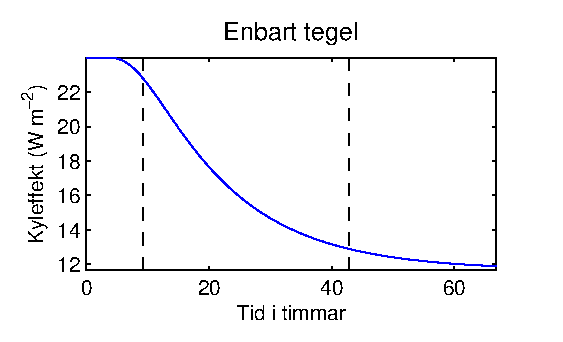
\includegraphics[width=6cm]{images/noinsulationstep.eps}
}\vspace{5mm}
\subfloat[Energiflöde ut från insidan av en vägg med $0,5\mbox{m}$ tegel och
$1\mbox{dm}$ tilläggsisolering bestående av mineralull.]{
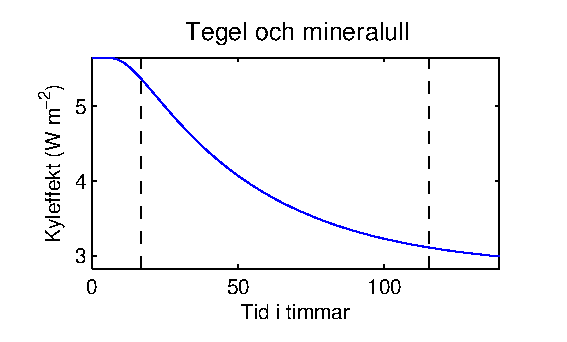
\includegraphics[width=6cm]{images/insulationstep.eps}
}
\caption{Energiflödet ut från insidan av en vägg där jämviktsläge med
$\unit[0]{^\circ C}$ på utsidan. Temperaturen förändras sedan
till $\unit[10]{^\circ C}$ vid tiden $t=0$. Insidan av väggen är satt till
konstanta $\unit[20]{^\circ C}$. De streckade linjerna markerar $\unit[10]{\%}$
fall samt $\unit[90]{\%}$ fall. Falltiden för dessa två väggar beräknades sedan
till $\unit[34,7704]{ timmar}$ för väggen utan isolering samt
$\unit[98,8372]{ timmar}$ för väggen med isolering. En annan intressant notering
är att det tog $\unit[9,5651]{ timmar}$ och $\unit[16,7533]{ timmar}$ för
energiflödet att falla $\unit[10]{\%}$. Beräkningarna är genomförda med finita
elementmetoden med $\unit[0,5]{m}$ tegel och $\unit[1]{dm}$ mineralull.}
\end{figure}


% \subsubsection{Luftfuktighetens inverkan på energiflöden}

\subsection{Luftflöde genom väggar – drag}

När det blåser på fastigheten får det luften kring fastigheten att cirkulera och även tränga in i 
byggnaden. När vinden ligger på med $\unit[3]{m/s}$, vinkelrätt mot nord- eller sydfasaden fås 
ett flöde som det i figur \ref{fig:windspeed} och trycket som då uppstår visas i figur 
\ref{fig:windpressure}. Tryckskillnaderna på de olika sidorna av husen kommer att driva 
ofrivillig ventilation vilket leder till energiförluster i form av infiltration.

\begin{figure}[hpbt]
\centering
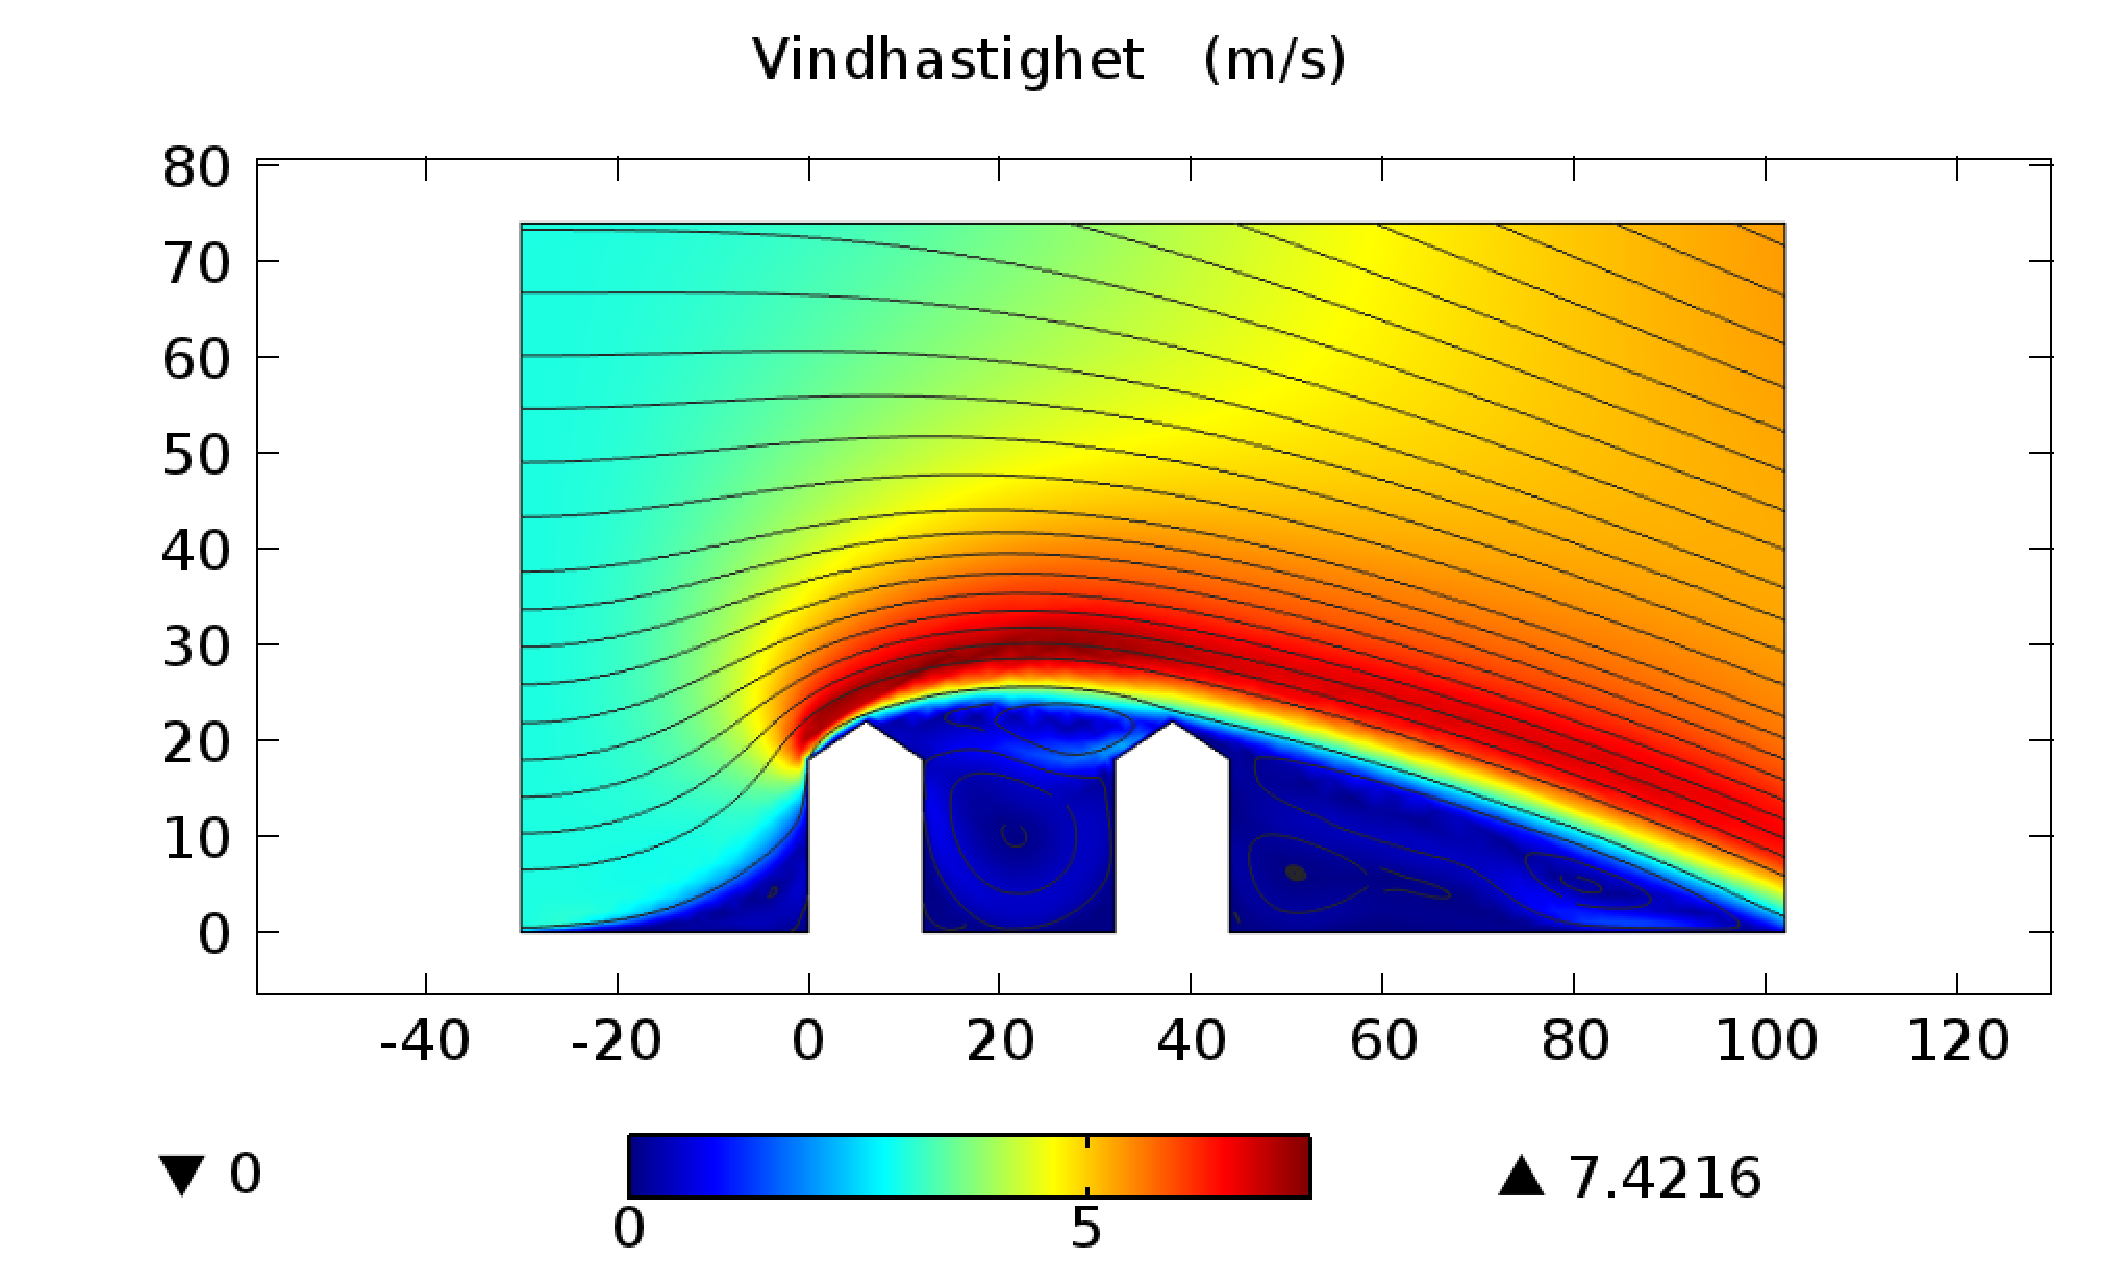
\includegraphics[width=127mm,height=76mm]{images/wind3mshdpi.eps}
\caption{\label{fig:windspeed}Vindhastiheten när vind i $\unit[3]{m/s}$ blåser mot fastigheten 
från vänster sida i figuren. Linjerna är strömlinjer och färgen indikerar farten. Värdena är 
framräknade med Comsol. Enhet m/s.}
\end{figure}


\begin{figure}[hpbt]
\centering
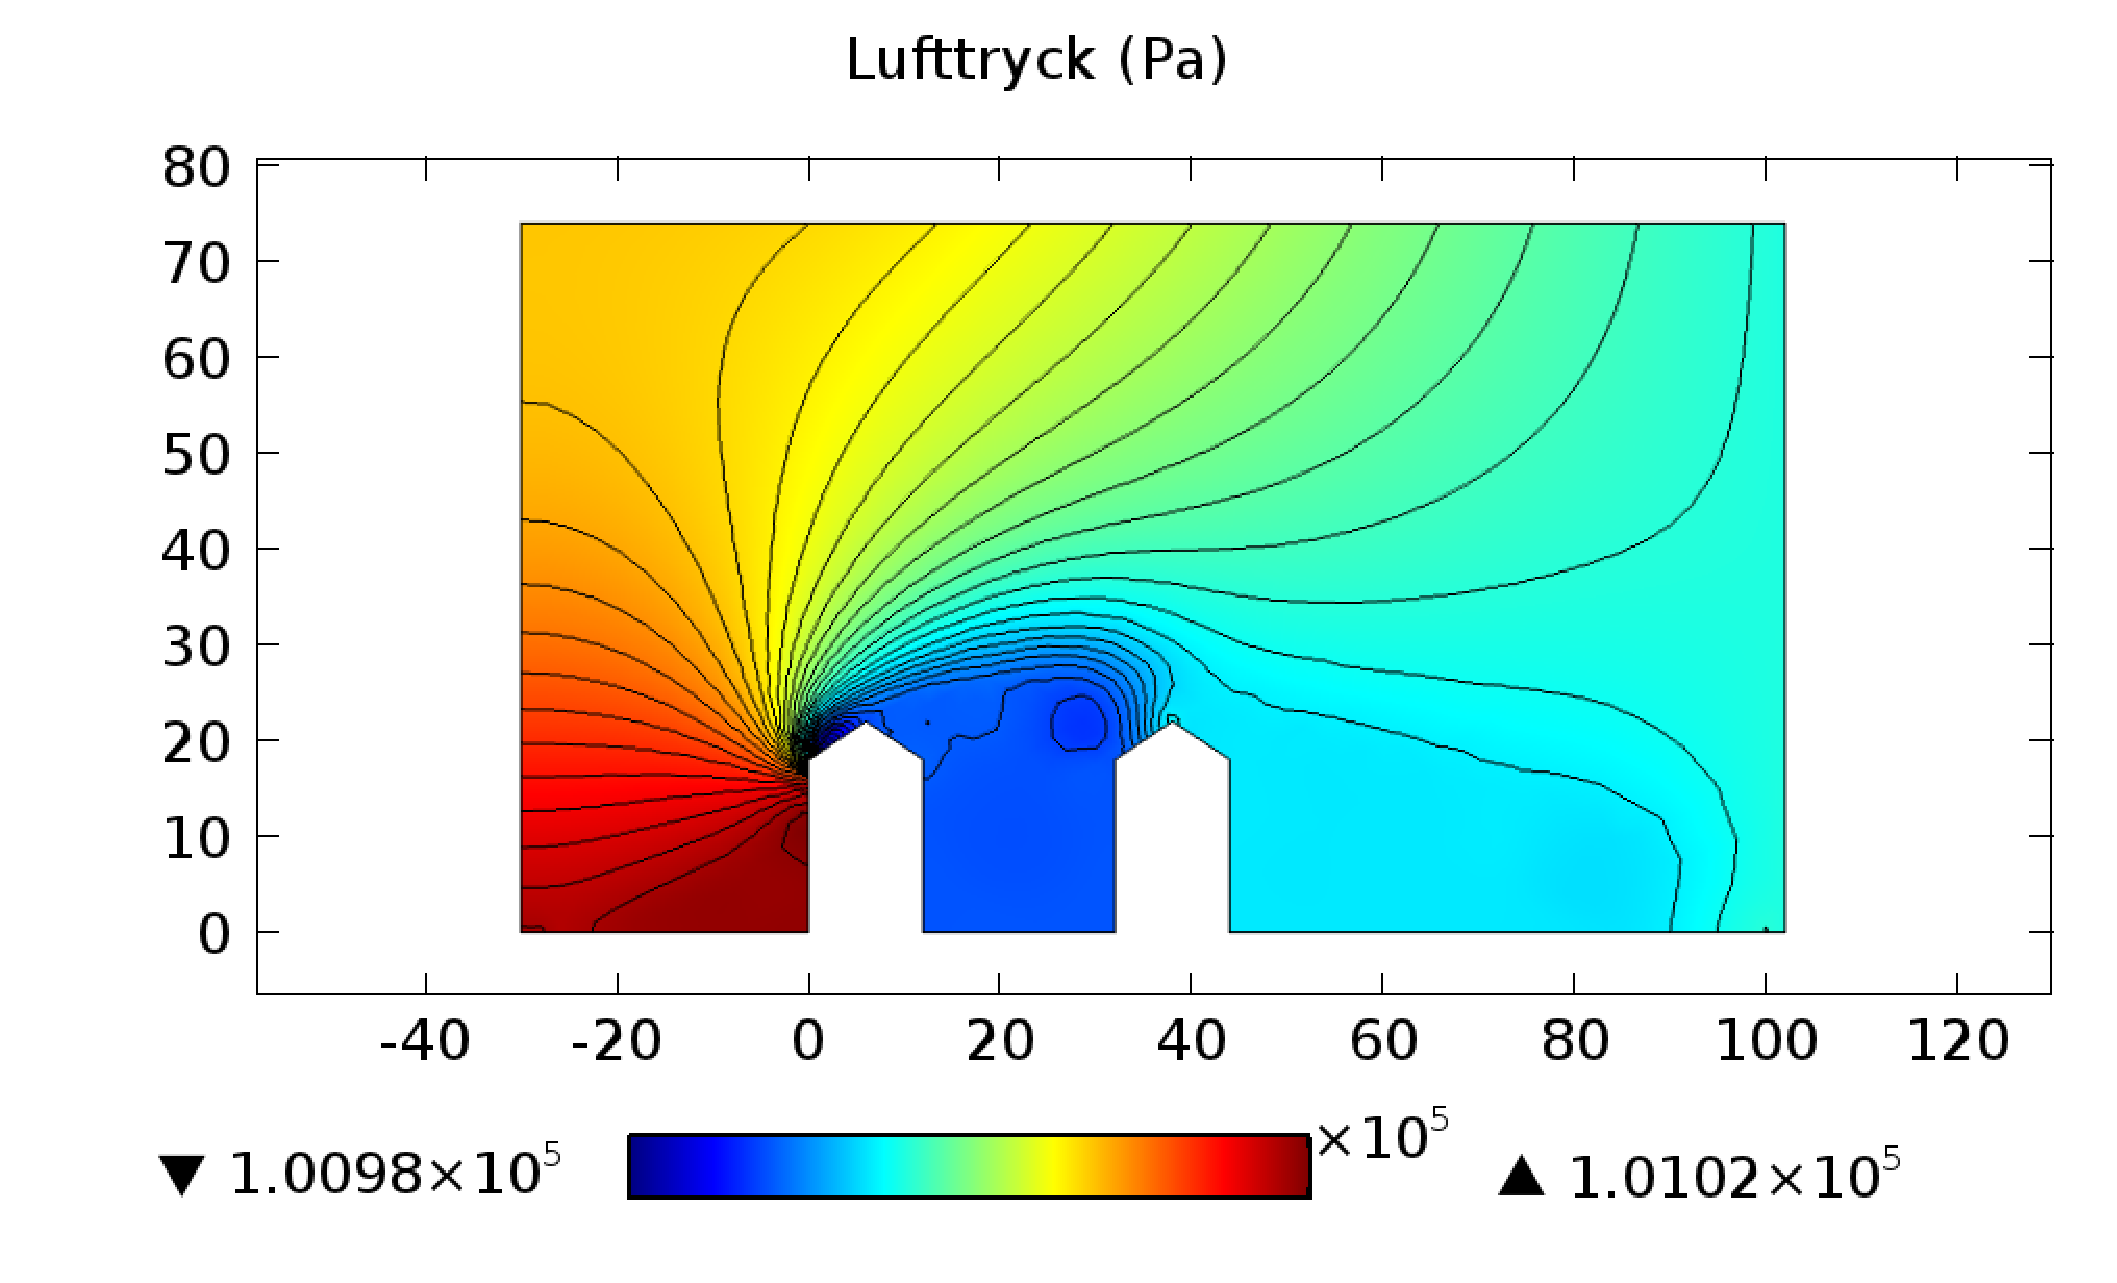
\includegraphics[width=127mm,height=76mm]{images/pressure3mshdpi.eps}

\caption{\label{fig:windpressure}Lufttrycket när vind i $\unit[3]{m/s}$ blåser mot fastigheten från vänster sida i figuren. Linjerna är isobarer, färgen indikerar lufttryck. Värdena är framräknade med Comsol. Enhet Pa.}
\end{figure}

% Resultat
Ur figur \ref{fig:windspeed} fås att det hus som ligger i lä utsätts inte för någon vind att tala om.
 Vidare fås ur figur \ref{fig:windpressure} att huset i lä utsätts för en betydligt mindre 
 tryckskillnad, än den byggnad som det blåser direkt på. I vårt exempel här, med en 
 vindhastighet runt $\unit[3]{m/s}$ fås en maximal tryckskillnad mellan norr- och sönderväggen 
 på 40 Pa, för fastigheten i lovart. Denna ökar när vindhastigheten ökar och vid 10 m/s fås en 
 tryckskillnad på 340 Pa för fastigheten i lovart. 

Applicerat på fastigheten på Walleriusgatan betyder detta att södervindar ger upphov till 
betydligt mer infiltrationsförluster än nordvindar. Till den aktuella byggnades fördel ska nämnas 
att södervindarna ofta är varmare än nordvindarna och de faktiska energiförlusterna blir 
troligen något mindre.

%%%%%%%%%%%%%%%%%%%%%%%%%%%%%%%%%%%%%%%%

Energiförlusterna på grund av drag har beräknats utifrån att en fix mängd energi per grad finns lagrad i en viss volym luft. Luftflödet genom väggen har beräknats på flera sätt. Både med Darcys lag och med byggfysikformeln, se avsnitt \ref{subsec:darcy}.

Energiförlusten har beräknats
  för en fastighet i lovart respektive en som ligger i lä av en annan byggnad, precis som 
  byggnaderna i figur \ref{fig:windspeed} och \ref{fig:windpressure}, vilket motsvarar att det 
  blåser på fastigheten på Walleriusgatan från söder respektive norr. Resultatet kan ses i figur 
  \ref{fig:windenergyloss} för en byggnad i lovart och en i lä samt för ett teoretiskt framtaget hus. Dessa två olika kurvor, framtagna med Darcys lag samt med en experimentell variant av densamma, får motsvara högsta respektive minsta gissningar för infiltrationsförluster i en byggnad.

Trycken är för figur \ref{fig:windenergylossa} och \ref{fig:windenergylossb} är framräknade för 
olika vindhastigheter med programmet Comsol medan det teoretiska modellen i figur 
\ref{fig:windenergylossc} är beräknat med med en approximation. 

Approximationen baserar sig
 på att tryckskillnaden mellan inne och ute är proportionerligt med vindhastigheten i kvadrat. Denna visar hur kyleffekten blir på en rätblocksformad byggnad som ligger helt ensam. Exakta kyleffekten beror väldigt mycket på vilken omgivning byggnaden står i.


\begin{figure}[hpbt]
\centering
\subfloat[\label{fig:windenergylossa}Byggnad som vinden blåser direkt på.]{
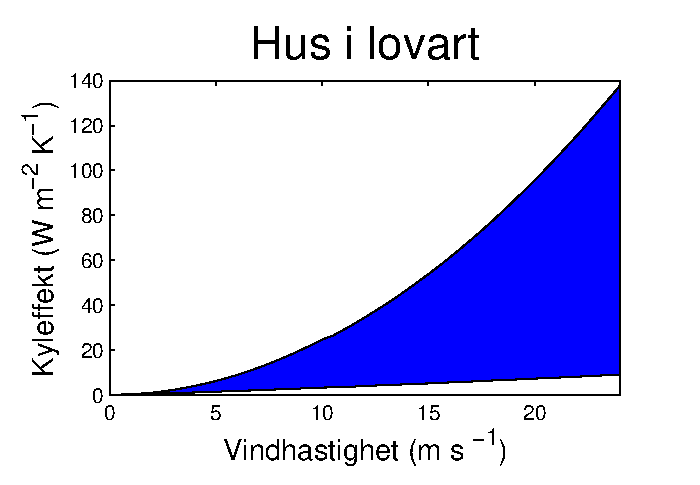
\includegraphics[width=60mm]{images/pressurewind.eps}}
\vspace{5mm}
\subfloat[\label{fig:windenergylossb}Byggnad som ligger i lä av en annan byggnad.]{
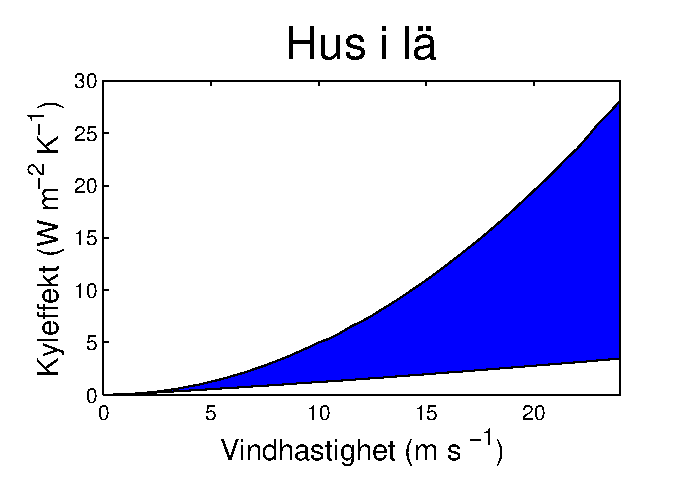
\includegraphics[width=60mm]{images/pressurenowind.eps}}

\subfloat[\label{fig:windenergylossc}Teoretisk approximation för lådformad byggnad.]{
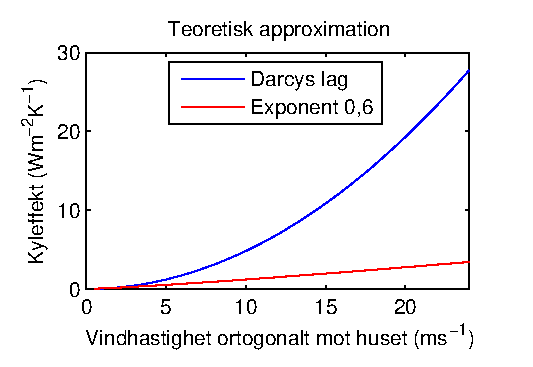
\includegraphics[width=60mm]{images/pressuretheory.eps}}

\caption{\label{fig:windenergyloss}Energiförlust per grad, max- respektive minvärde.
Framtaget med Comsol (a och b) och teoretiskt framräknade med en approximation (c).}
\end{figure}

% Resultat
Vilken kyleffekt vinden har på fastigheten är mer osäkert vid högre vindhastigheter. När vinden
 ligger på med upp emot 25 m/s kan kyleffekten variera från några tiotal watt per Kelvin upp 
 emot drygt hundra. Motsvarande kan kyleffekt för ett hus i lä vara mellan några watt per 
 Kelvin upp mot knappt trettio. För det teoretiskt beräknade huset fås även där att kyleffekten 
 kan vara mellan några watt per Kelvin upp mot knappt trettio dito. När vi har mer normala 10 
 m/s ser vi istället att kyleffekten kan vara från några få upp emot 20 W/K för en byggnad i 
 lovart, och ungefär en fjärdedel av det för en byggnad i lovart.



\subsection{Solstrålning genom fönster}

Exempel på resultat från beräkningar på solstrålning genom fönster. Beräknat via trial.m i code-mappen.

I figur \ref{fig:sun0101and0601} ses de relevanta vinklar som bildas av solens position den första april, 2012. Den blå linjen i figuren representerar solens vinkel relativt ett fönsters normal (då denna pekar i horisontell sydlig riktning) och kan användas för att uppskatta effekten som solinstrålning bidrar till. Om solens intensitet antas vara konstant $\unit{200}{W/m^2}$ beräknas denna effekt motsvara vad som visas i figur \ref{fig:effekt0101and0601}. Här antas fönstrets area uppgå till $\unit{1.5}{m^2}$, g-värdet för normal solstrålning är ? och värdet p i koden sätts till ?, ty fönstren i den avsedda byggnaden är av typ treglas utan ytbeläggningar.

\begin{figure}[hpbt]
\centering
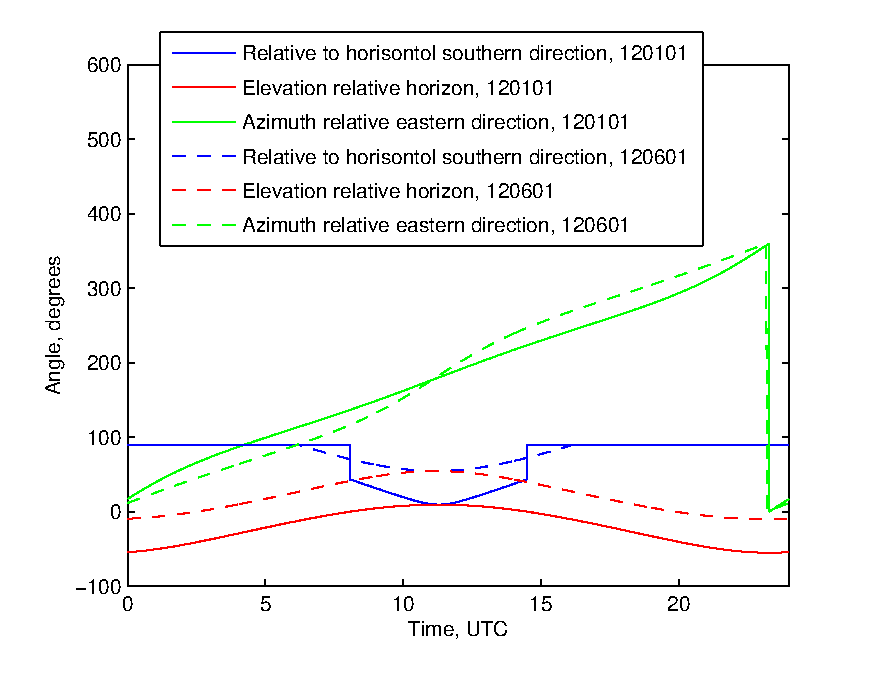
\includegraphics[scale=1]{images/sun0101and0601.eps}
\caption{\label{fig:sun0101and0601} Beräknade vinklar vid Walleriusgatan den första januari 2012 samt den första juni samma år, tid i UTC}
\end{figure}

\begin{figure}[hpbt]
\centering
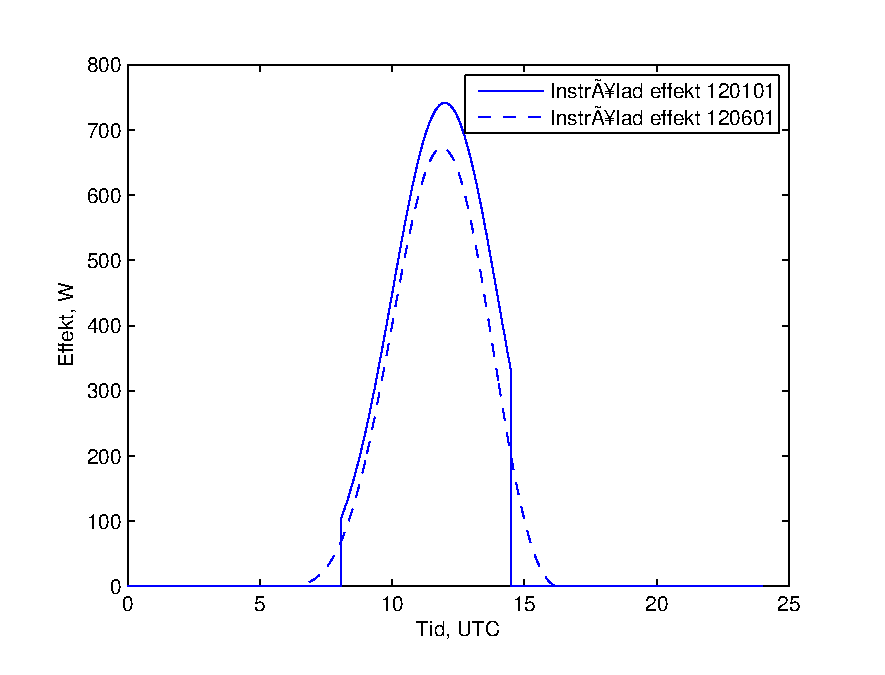
\includegraphics[scale=1]{images/effekt0101and0601.eps}
\caption{\label{fig:effekt0101and0601} Beräknad effekt genom ett fönster vars normal pekar i horisontella sydriktningen, den första januari 2012 samt den första juni samma år. Solens intensitet varierar under dagen enligt den blå kurvan.}
\end{figure}


\section{Energiflöde genom grunden}

% \subsubsection{Flöde vid termisk jämvikt}

Vid beräkningen av värmeflödet genom grunden användes geometrin som kan ses i figur \ref{fig:groundheat}.
Källaren antas vara belägen en halv meter under marknivån.

Som kan ses så varierar ej energiflödet så mycket mellan årstiderna och antags därför vara konstant i många applikationer.


\emph{\color{red} Nedanstående text måste göras om med de nya figurerna i åtanke,}
I samma figur ses även temperaturfördelningen vid termisk jämvikt då markens temperatur långt under huset sätts till konstanta $\unit[8]{^{circ}C}$. Vid markytan sattes konvektionskoefficienten till $h=\unit[15,5]{Wm^{-2}K^{-1}}$, motsvarande en ungefärlig vindhastighet (parallel med ytan) på $\unit[2]{ms^{-1}}$ vid utomhustemperaturen $\unit[0]{^{\circ}C}$. Källarens temperatur antas vara konstant $\unit[10]{^{\circ}C}$ och \textcolor{red}{grundens U-värde approximeras till $\unit[?]{Wm^{-2}K^{-1}}$}.


\begin{figure}
\centering
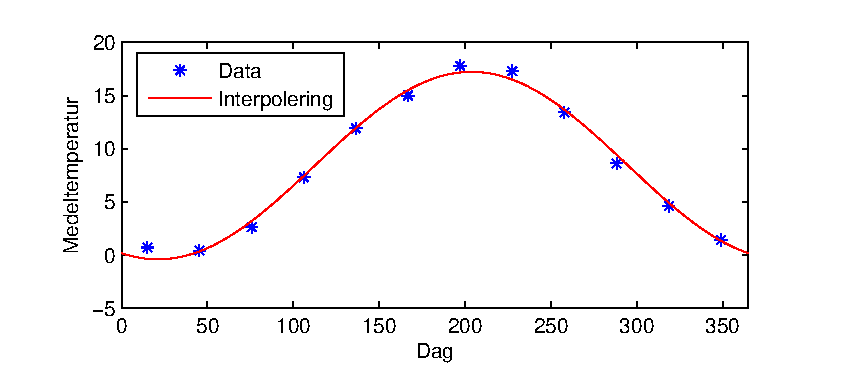
\includegraphics{images/meantemperature.eps}
\caption{Medeltemperaturen för göteborg de senaste 20 åren. Punkterna är data tagna från Miljöförvaltningen
och linjen är minstakvadratanpassningen som senare använts för att beräkna energiflöden.
\emph{\color{red} Denna graf kanske inte ska ligga här eller alls vara med. Metod möjligtvis? Vad tycker ni?}}
\end{figure}

\begin{figure}
\centering
\subfloat[Temperaturfördelningen i $^\circ\mbox{C}$ första januari.]{
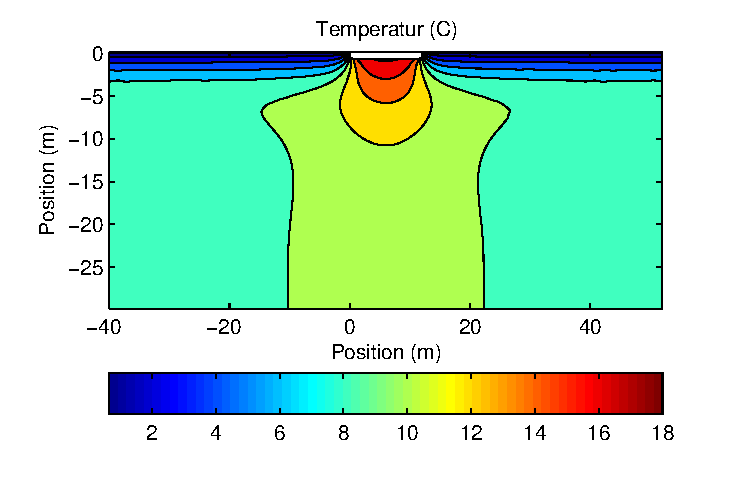
\includegraphics{images/groundheatdec.eps}
}

\subfloat[Temperaturfördelningen i $^\circ\mbox{C}$ första juli.]{
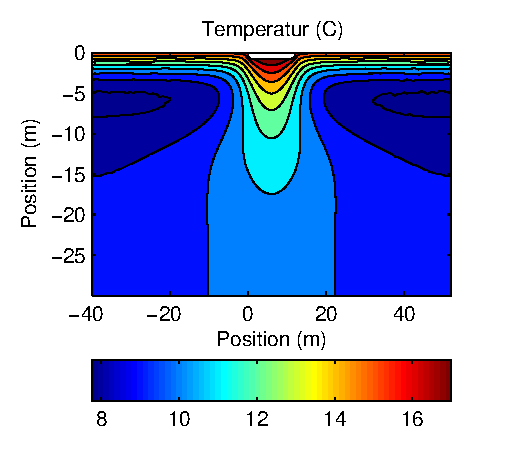
\includegraphics{images/groundheatjune.eps}
}
\caption{\label{fig:groundheat}Temperaturen i marken under en byggnad angivet i grader Celsius.
Temperaturfördelningarna skall motsvara två fiktiva dagar under ett år som är baserad på månadsmedeltemperaturen
de senaste 20 åren i Göteborg. Konvektionsparametern är satt till $h=15,5$. }
\end{figure}


\begin{figure}
\centering
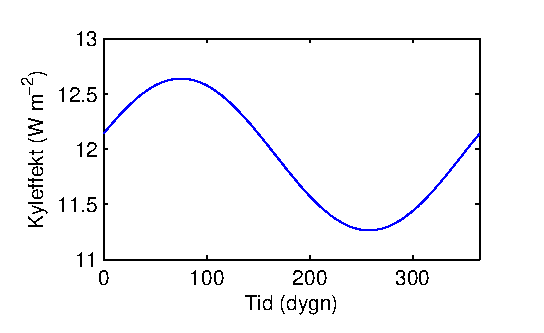
\includegraphics{images/groundcool.eps}
\caption{Kyleffekten per $m^2$ från grunden för medelåret de senaste tjugo åren. \emph{\color{red} Samma parametrar som figuren ovan.}\emph{\color{red}                                     
Detta är en viktig figur. Här kan ses att $\Delta Q = 1.5*22*13 = \unit[439]{W}$. Detta offsettas lätt genom att fler
människor befinner sig i fastigheten på vintern ty det är kallt ute eller fler kollar på tv istället för att sola.
Således finns det inget behov för att reglera framlednigstemperaturen för energiförluster från grunden. Kan antagas konstant
$\approx \unit[3,5]{kW}$. Låter denna siffra rimlig?}}

\end{figure}


% \subsubsection{Flöde vid transient förlopp}

Vid beräkningen av energiflödet genom grunden användes geometrin som kan ses i figur~\ref{fig:groundheat}. Källaren antas vara belägen en halv meter under marknivån. I resonomanget nedan kommer det att visa sig att marken reagerar så pass långsamt på temperaturförändringar att jämviktsläget är det enda relevanta. Ett transient förlopp är helt enkelt långt ifrån verkligheten.

Som kan ses i figur~\ref{fig:cooling_ground} så varierar inte energiflödet mer än en dryg watt per kvadratmeter mellan årstiderna och i många applikationer antas det därför vara konstant. Då vår grund är ungefär $\unit[22]{m}\cdot\unit[13]{m}=\unit[286]{m^2}$ ger detta ett energiutflöde mellan $\unit[3,6]{kW}$ på våren och $\unit[3,2]{kW}$ under tidig höst. 

\begin{figure}
\centering
\subfloat[Temperaturen i marken den första januari, $^\circ\mbox{C}$.]{
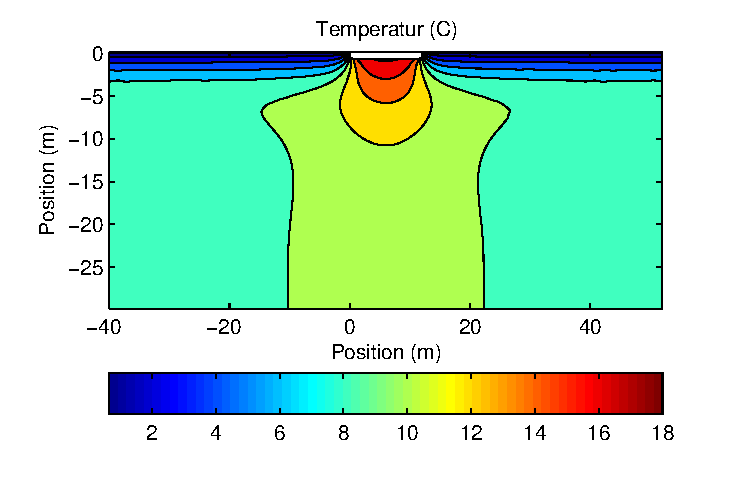
\includegraphics[width=7cm]{images/groundheatdec.eps}
}
\subfloat[Temperaturen i marken den första juli, $^\circ\mbox{C}$.]{
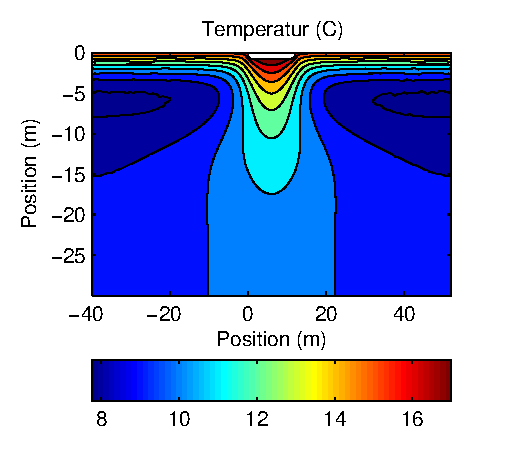
\includegraphics[width=7cm]{images/groundheatjune.eps}
}
\caption{\label{fig:groundheat}
Temperaturen i marken under byggnaden, $\unit{^\circ C}$, beräknat utifrån månadsmedeltemperaturen de senaste 20 åren i Göteborg för två fiktiva dagar i juni respektive januari. Konvektionsparametern är satt till $h=15,5$. }
\end{figure}


\begin{figure}
\centering
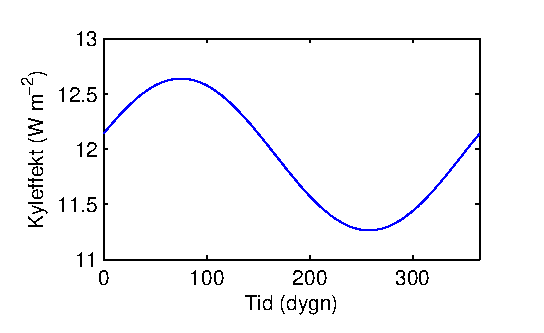
\includegraphics{images/groundcool.eps}
\caption{\label{fig:cooling_ground}
Kyleffekten per kvadratmeter från grunden för medelåret de senaste tjugo åren. Konvektionsparametern är satt till $h=15,5$. }

\end{figure}


